\DiaryEntry{Maximum Flow, Definitions and Basics}{2020-05-27}{Algorithms}

\subsection{Definitions}

A flow network $G = (V,E)$ is a directed graph in which each edge $(u,v) \in E$ has a non-negative capacity $c(u,v) \geq 0$ assigned to it. To simplify expressions, we use the convention that if there is no edge between two vertices $u,v$ then the corresponding capacity is zero, $c(u,v) = $. There is the restriction that if there is an edge $(u,v)$, there is no edge $(v,u)$ in the reverse direction. There are two special vertices in the graph; a source vertex $s$ and a sink vertex $t$.

With this in place, we can formally define flows. A flow in $G$ is a real-valued function $V \times V \rightarrow \mR$ that satisfies the following two properties:

\begin{description}
\item [Capacity Constraint:] The flow along each edge has to be lower than the edge capacity. That is, for all $u,v \in V$, we require $0 \leq f(u,v) \leq c(u,v)$.
\item [Flow Consideration:] For all vertices but $s$ and $t$, the sum of all incoming flows is equal the sum of all outgoing flows. In other words, no flow is or created at the vertices. Formally, we have that fFor all $u \in V - \{s,t\}$, we require

\bee
\sum_{v \in V} f(v,u) = \sum_{v \in V} f(u,v)
\eee

\end{description}

We also define the value $|f|$ of a flow as

\bee
|f| = \sum_{v \in V} f(s,v) - \sum_{v \in V} f(v,s)
\eee

Note that normally, no flow is going \emph{towards} the source $s$; i.e. the second sum is zero.

In the maximum-flow probem, we are given a flow network with a source vertex $s$ and sink $t$, and we want to find a flow of maximum value.

\paragraph{Example.} The following Figure shows an example flow network. The labels of the edges follow the convention $f(u,v)/c(u,v)$. So for example, the capacity on the edge $(2,1)$ is $4$, the actual flow along this egde is $1$. 

\begin{figure}[H]
\centering
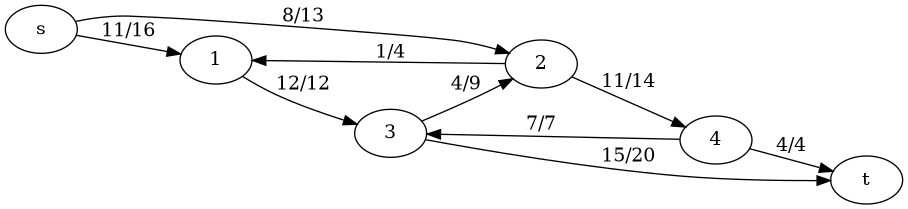
\includegraphics[scale=0.45]{images/max_flow_01.png}
\end{figure}


\subsection{Ford-Fulkerson Method}

The Ford-Fulkerson Method solves the maxium-flow problem. It is a method and not an algoritmh, as it provides several implementation options. Ford-Fulkeron is based on three ideas: Residual networks, augmenting paths, and cuts.

The method iteratively increases the value of the flow. We start with $f(u,v)=0$ for all $u,v \in V$, giving an initial flow of value of $0$. At each iteration, we increase the flow value by finding an ``augmenting'' path in an associated ``residual network'' $G_f$.

Once we know the edges of an augmenting path in $G_f$ , we can easily identify specific edges in $G$ for which we can change the flow so that we increase the value of the flow. Although each iteration of the Ford-Fulkerson method increases the value of the flow, we shall see that the flow on any particular edge of $G$ may increase or decrease; decreasing the flow on some edges may be necessary in order to enable an algorithm to send more flow from the source to the sink. We repeatedly augment the flow until the residual network has no more augmenting paths. The max-flow min-cut theorem will show that upon termination, this process yields a maximum flow.

The Ford-Fulkerson Method looks as follows

\begin{Verbatim}[numbers=left, xleftmargin=5mm]
Ford-Fulkerson(G,s,t)
   initialize flow f to 0
   while there exists an augmenting path p in the residual network G_f
      augment flow f along p
   return f
\end{Verbatim}


\subsubsection{Residual Networks}

Given a flow network $G$ and a flow $f$, the residual network $G_f$ consists of the vertices of $G$ and edges with capacities that can change the flow on edges in $G$.

We consider each edge independently: An edge can take additional flow if the flow along the edge is below the edge's capacity; in this case, it can take the difference between capacity and flow. If the difference is positive, the edge is placed into $G_f$ with a ``residual capacity'' $c_f(u,v) = c(u,v) - f(u,v)$. We place only edges in $G_f$ which can take additional flow; i.e. ones where $c_f(u,v) > 0$. Edges which already carry a flow equal their capacity, where $c_f(u,v) = 0$ are not added to $G_f$.

Besides that, the residual network $G_f$ may contain edges not in $G$. As the Ford-Fulkerson algorithm proceeds, it may need to decrease fow along an edge. In order to represent a possible flow decrease along an edge, we place an edge in the reverse direction, $(v,u)$ with residual capacity $c_f(v,u) = f(u,v)$ in the residual network $G_f$. At maximum, a flow along this edge can cancel out the flow present in $G$.

To formalize, we have a flow network $G = (V,E)$ with source $s$ and sink $t$. Let $f$ be a flow in $G$, and two vertices $u,v \in V$. The residual capacity $c_f(u,v)$ is then defined according to

\bee
c_f(u,v) = \begin{cases} c(u,v) - f(u,v) & \text{if } (u,v) \in E \\
  f(v,u) & \text{if } (v,u) \in E \\
  0 & \text{otherwise}
\end{cases}
\eee

Note that notation is a bit tricky here: If we have an edge from $u$ to $v$, the residual capacity \emph{from $u$ to $v$} is $c(u,v) - f(u,v)$, but there is also a residual capacity \emph{from $v$ to $u$} equal to $f(u,v)$. This residulal capacity allows to completely cancel the flow $u$ to $V$.

The corresponding residual network of $G$ induced by flow $f$ is $G_f(V, E_f)$ where

\bee
E_f = \{ (u,v) \in V \times V: c_f(u,v) > 0 \}
\eee

Note that this is not a flow network, as it may contain an edge $(u,v)$ and the reverse edge $(u,v)$.

\paragraph{Example.} Continuing our example, we obtain the following residual network. As an example, consider the edge $(2,4)$ with flow $f(2,4) = 11$ and capacity $c(2,4) = 14$. The residual flow from $2$ to $4$ is therefore $c_f(2,4) = 3$ (that's the value before the link saturates). In the reverse direction we can increase the flow up to $f(2,4) = 11$, so we have $c_f(4,2) = 11$. Therefore, the residual network has an edge $(2,4)$ and an edge $(4,2)$.


\begin{figure}[H] \centering
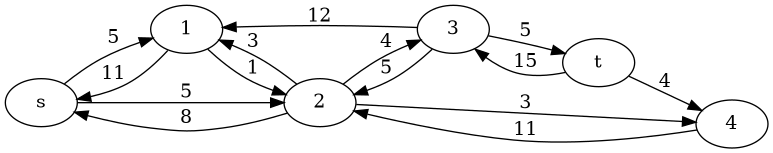
\includegraphics[scale=0.5]{images/max_flow_02.png}
\end{figure}


The residual network has the same properties as a flow network. We can also define a flow in a residual network, however, the flow needs to consider the capacities of the residual network.

If $f$ is a flow in $G$ and $f'$ is a flow in the corresponding residual network $G_f$, we define the augmentation of flow $f$ by $f'$, denoted by $f \uparrow f'$, to be a function from $V \times V \rightarrow \mR$, defined by

\bee
(f \uparrow f')(u,v) = \begin{cases} f(u,v) + f'(u,v) - f'(v,u) & \text{if } (u,v) \in E \\
  0 & \text{otherwise}
  \end{cases}
\eee


\begin{theorem}
  Let $f$ be a flow on $G$, $G_f$ be a residual network of $G$ induced by $f$, and let $f'$ be a flow in $G_f$. Then the function $f \uparrow f'$ is a flow in $G$ with value $|f + f'| = |f| + |f'|.$
\end{theorem}

Proof is omitted.

\subsubsection{Augmenting Paths}

An augmenting path $p$ on a graph $G$ with flow $f$ is a simple path from $s$ to $t$ in the residual network $G_f$. As described in the previous section, we may increase the flow on an edge $(u,v)$ of an augmenting path by up to $c_f(u,v)$ without violating the capacity constraint on $(u,v)$ or $(v,u)$ (whicever edge is in the original flow network $G$).

We can increase the flow on the path $p$ by the minimum residual capacity on the path; we call this vaslue the residual capacity of $p$. Formally it is defined by

\bee
c_f(p) = \min_{(u,v) \in p} c_f(u,v)
\eee

We now have the following theorem.

\begin{theorem}
  We have a flow network $G$ with flow $f$  and an augmenting path $p$ in $G_f$. Define a function $f_p:V\times V \rightarrow \mR$ according to

  \bee
  f_p(u,v) = \begin{cases} c_f(p) & \text{if } (u,v) \in p \\
    0 & \text{otherwise}
    \end{cases}
  \eee

  Then $f_p$ is a flow in $G_f$ with value $|f_p| = c_f(p) > 0$. If we augment $f$ by $f_p$, then $f \uparrow f_p$ is a flow in $G$ with value $|f \uparrow f_p| = |f| + |f_p| > |f|$.
\end{theorem}

The last part is the most interesting one; it states that if we augment $f$ by $f_p$, we get a flow which is closer to the maximum flow.

\paragraph{Example.} Let's choose an augmenting path in our residual network. We take a path along vertices $s - 2 - 3 - t$. The residual capacity of this path is $\min\{5, 4, 5\} = 4$, that is we can increase the capacity by $4$ units. 

The Figure below shows the updated flow network. The flows along the vertices $s - 2 - 3 - t$ has been increased by the residual capacity of the augmenting path.

\begin{figure}[H]
\centering
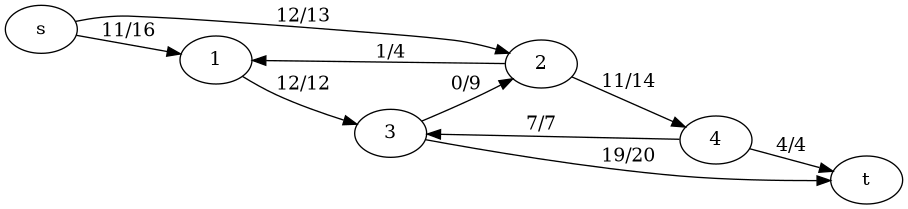
\includegraphics[scale=0.45]{images/max_flow_04.png}
\end{figure}



\subsubsection{Cuts of Flow Networks}

The previous theorem shows that repeatedly augmenting path increases the flow. The question is when we have found an optimum; i.e. what is the maximum achievable flow? The max-flow min-cut theorem gives an answer to this question.

A cut in a flow network partitions the vertices into two sets $S, T = V - S$ with $s \in S$ and $t \in T$. Given a flow, we can calculate the net flow across the cut as follows,

\bee
f(S,T) = \sum_{u \in S} \sum_{v \in T} f(u,v) - \sum_{u \in S} \sum_{v \in T} f(v,u)
\eee

The capacity of the cut is given as the sum of capacity of all edges across the cut,

\bee
c(S,T) = \sum_{u \in S} \sum_{v \in T} c(u,v)
\eee

Note the asymmetry in the definitions: The flow considers the difference betwen flow from $S$ to $T$ and $T$ to $S$; whereas the capacity is the capacity of alllinks from $S$ to $T$.

A minimum cut of a network is a cut whose capacity is minium over all cuts of the network.

\paragraph{Example.} Continuing with our example, the following Figure shows a cut $S-T$ in red. Set $S$ contains vertices $s,1$, set $T$ contains vertices $2,3,4,t$. The net flow across the cut is

\bee
f(S,T) = 8 - 1 + 12 = 19 
\eee

Had we chosen the cut more to the left (shown in dotted red), we have the same net flow, $f(S,T) = 8 + 11 = 19$; in a similar spirit, for the cut on the right (shown in dotted green), the net flow is again $f(S,T) = 11 - 7 + 15 = 19$.

The capacity of the cut is

\bee
c(S,T) = 13 + 12 = 25
\eee

However, this is not the min-cut. The Figure shows the min-cut in blue. Its capacity is $12 + 9 + 4 = 25$.


\begin{figure}[H] \centering
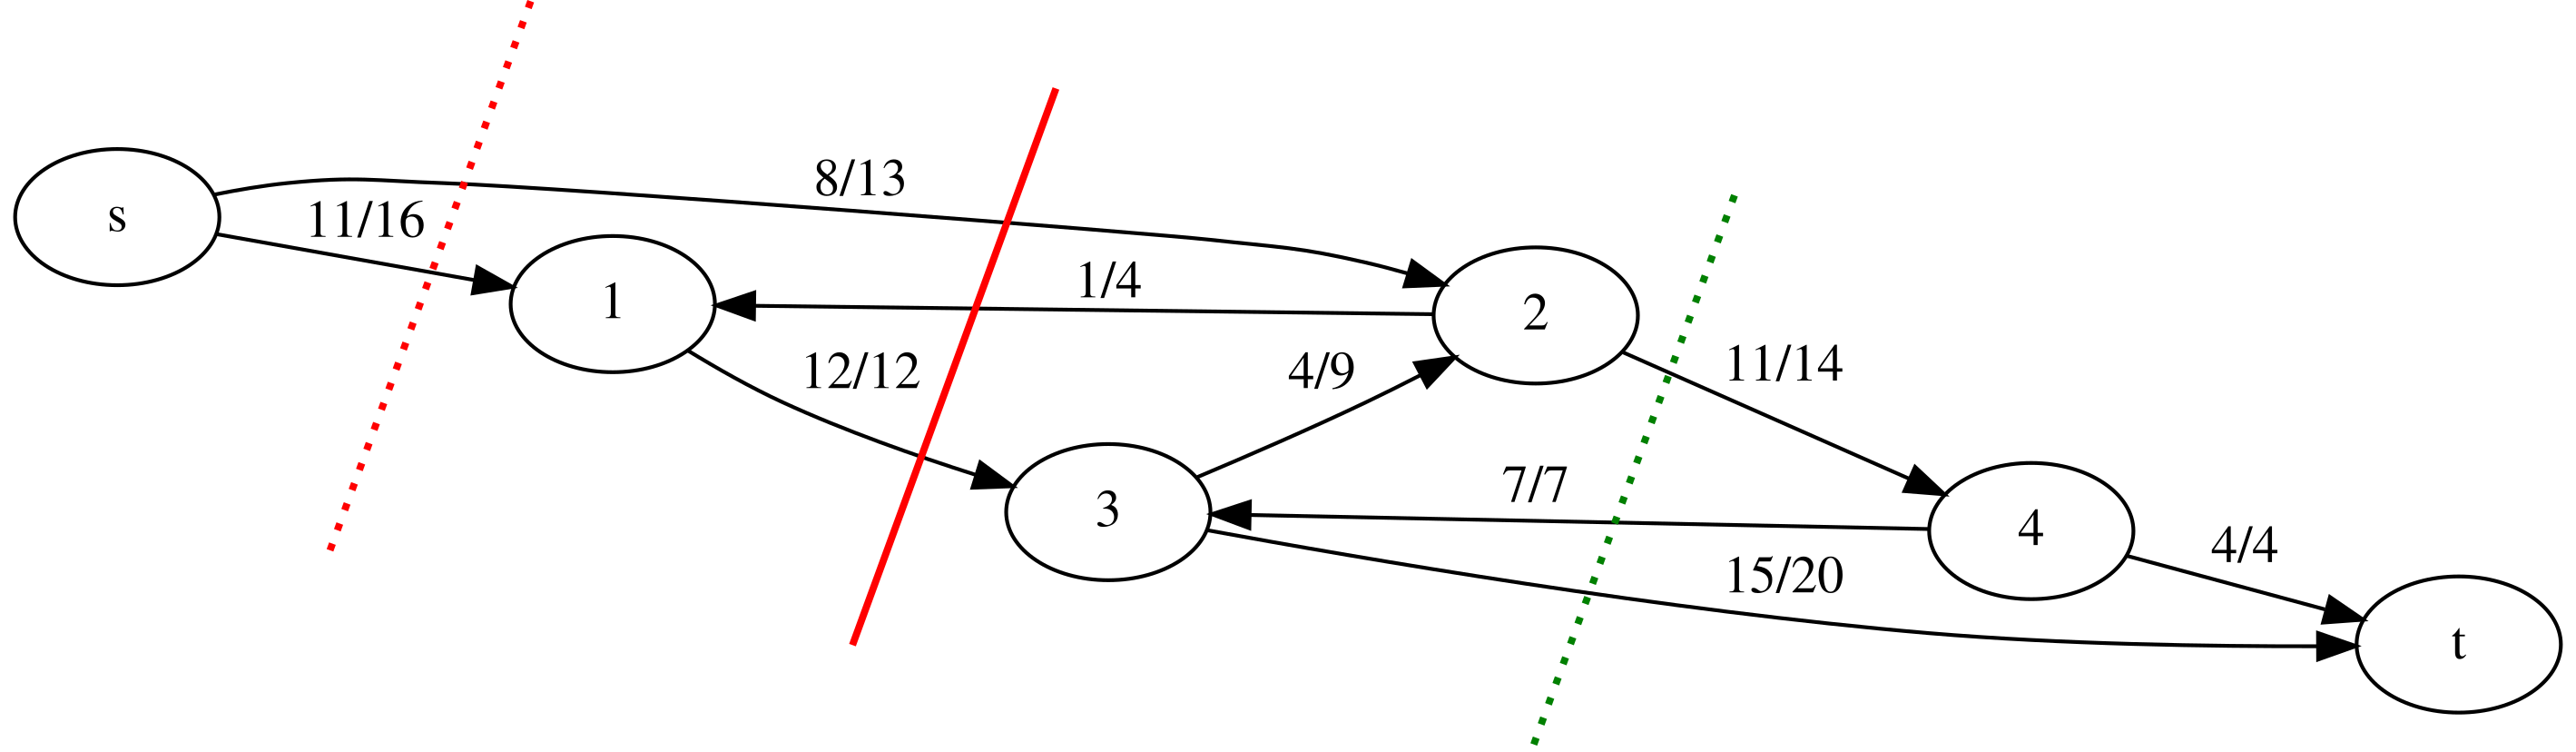
\includegraphics[scale=0.6]{images/max_flow_03.png}
\end{figure}


The following theorem shows that the netflow associated with a cut is actually indepenedent of where the cut is taken.

\begin{theorem}
  Let $f$ be a flow in a flow network $G$ and let $(S,T)$ be any cut of $G$. Then the net flow across $(S,T)$ is $|f|$; in particular it is indepenent of the cut.
\end{theorem}

Intuitively, the theorem is clear: In a flow network, all vertices but $s$ and $t$ do not create/destroy flow. Therefore, if $s$ is one side of the cut and $t$ on the other, the flow does not depend on the actual postion of the cut. 

We can use cut capacities to bound the value of a flow using the following theorem.

\begin{theorem}
  The value of any flow $f$ in a flow network $G$ is bounded above by the capacity of any cut of $G$.
\end{theorem}

While the above theorem provides a bound, the following max-flow min-cut theorem actually states that the maximum flow in a network equals the capacity of a minimum cut of the network.

\begin{theorem}[Max-flow Min-cut Theorem]
  If $f$ is a flow in a flow network $G$ with source $s$ and sink $t$, the following conditions are equivalent
  \begin{itemize}
  \item $f$ is a maximum flow in $G$.
  \item The residual network $G_f$ contains no augmenting paths.
  \item The flow $|f|$ equals the flow across a cut: $|f| = c(S,T)$ for any cut $(S,T)$ of $G$.
  \end{itemize}
\end{theorem}

We omit the proof of this theorem.

\subsection{Basic Ford-Fulkerson Algorithm}

We now extend the Ford-Fulkerson method to a more concrete algorithm. Every egdge tracks the flow via an attribute , $(u,v).f$. The algorithm finds ``some suitable'' augemting path $p$ and use it to modify the flow $p$. As the previous discussions show, we replace $f$ by $uparrow f_p$ and obtain a new flow with value $|f| + |f_p|$.  

The algorithm is as follows.

\begin{Verbatim}[numbers=left, xleftmargin=5mm]
Ford-Fulkerson(G,s,t)
   for each edge (u,v)
      (u,v).f = 0
   while there exists an augmenting path p in the residual network G_f
      c_f(p) = min c_f(u,v) for (u,v) in p
      for each edge (u,v) in p
         if (u,v) in E
            (u,v).f = (u,v).f  + c_f(p)
         else
            (u,v).f = (v,u).f - c_f(p)   
   return f
\end{Verbatim}

The tricky part is how to obtain / select augmenting paths. If the augmenting paths are chosen in the ``wrong'' order the algorithm may take longer to converge and / or not converge at all.

In the following example, we show an order where the optimum is achieved.

The left Figure in (a) shows the input graph (our running example, but witha different layout) and a shaded augemting path. The residual capacity of the path is $4$; the left Figure in (a) shows the resulting residual network: The flow along the augmenting path is $4$, all other flows are (still) zero. In (b) another augmenting path is chosen (left); the result is shown on the right.

\begin{figure}[H] \centering
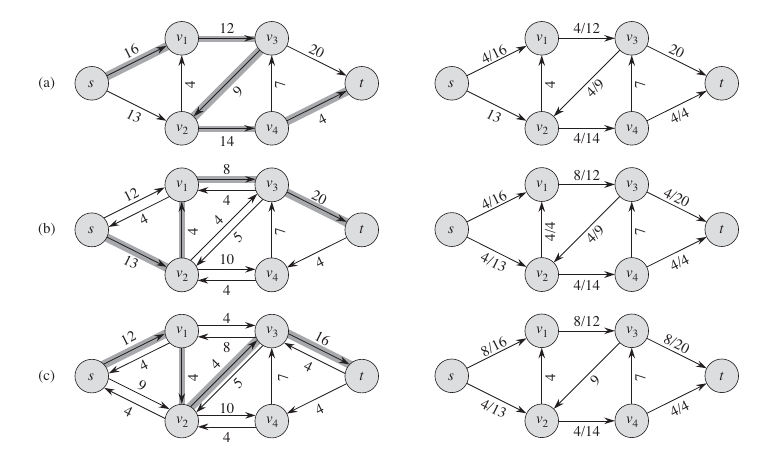
\includegraphics[scale=0.5]{images/max_flow_ex_1.png}
\end{figure}

We contine with (d) and (e). Figure (f) shows a flow network with no further augmenting path. Therefore, the flow network in the right Figure of (e) shows the maximum flow which equals $23$. Since no further augmenting path exists, the algorithm stops here.

\begin{figure}[H] \centering
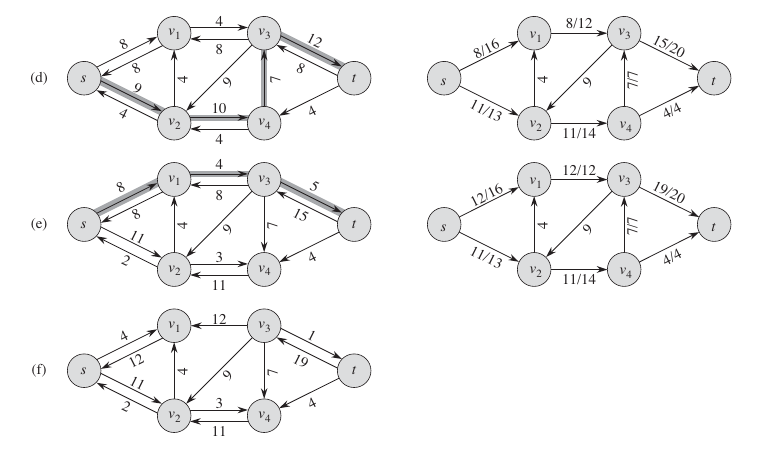
\includegraphics[scale=0.5]{images/max_flow_ex_2.png}
\end{figure}



%%% Local Variables:
%%% mode: latex
%%% TeX-master: "journal"
%%% End:
